\documentclass[10pt, a5paper]{article}
\usepackage{pdfpages}
\usepackage{parallel}
\usepackage[T2A]{fontenc}
\usepackage{ucs}
\usepackage[utf8x]{inputenc}
\usepackage[polish,english,russian]{babel}
\usepackage{hyperref}
\usepackage{rotating}
\usepackage[inner=2cm,top=1.8cm,outer=2cm,bottom=2.3cm,nohead]{geometry}
\usepackage{listings}
\usepackage{graphicx}
\usepackage{wrapfig}
\usepackage{longtable}
\usepackage{indentfirst}
\usepackage{array}
\newcolumntype{P}[1]{>{\raggedright\arraybackslash}p{#1}}
\frenchspacing
\usepackage{fixltx2e} %text sub- and superscripts
\usepackage{icomma} % коскі ў матэматычным рэжыме
\PreloadUnicodePage{4}

\newcommand{\longpage}{\enlargethispage{\baselineskip}}
\newcommand{\shortpage}{\enlargethispage{-\baselineskip}}

\def\switchlang#1{\expandafter\csname switchlang#1\endcsname}
\def\switchlangbe{
\let\saverefname=\refname%
\def\refname{Літаратура}%
\def\figurename{Іл.}%
}
\def\switchlangen{
\let\saverefname=\refname%
\def\refname{References}%
\def\figurename{Fig.}%
}
\def\switchlangru{
\let\saverefname=\refname%
\let\savefigurename=\figurename%
\def\refname{Литература}%
\def\figurename{Рис.}%
}

\hyphenation{admi-ni-stra-tive}
\hyphenation{ex-pe-ri-ence}
\hyphenation{fle-xi-bi-li-ty}
\hyphenation{Py-thon}
\hyphenation{ma-the-ma-ti-cal}
\hyphenation{re-ported}
\hyphenation{imp-le-menta-tions}
\hyphenation{pro-vides}
\hyphenation{en-gi-neering}
\hyphenation{com-pa-ti-bi-li-ty}
\hyphenation{im-pos-sible}
\hyphenation{desk-top}
\hyphenation{elec-tro-nic}
\hyphenation{com-pa-ny}
\hyphenation{de-ve-lop-ment}
\hyphenation{de-ve-loping}
\hyphenation{de-ve-lop}
\hyphenation{da-ta-ba-se}
\hyphenation{plat-forms}
\hyphenation{or-ga-ni-za-tion}
\hyphenation{pro-gramming}
\hyphenation{in-stru-ments}
\hyphenation{Li-nux}
\hyphenation{sour-ce}
\hyphenation{en-vi-ron-ment}
\hyphenation{Te-le-pathy}
\hyphenation{Li-nux-ov-ka}
\hyphenation{Open-BSD}
\hyphenation{Free-BSD}
\hyphenation{men-ti-on-ed}
\hyphenation{app-li-ca-tion}

\def\progref!#1!{\texttt{#1}}
\renewcommand{\arraystretch}{2} %Іначай формулы ў матрыцы зліпаюцца з лініямі
\usepackage{array}

\def\interview #1 (#2), #3, #4, #5\par{

\section[#1, #3, #4]{#1 -- #3, #4}
\def\qname{LVEE}
\def\aname{#1}
\def\q ##1\par{{\noindent \bf \qname: ##1 }\par}
\def\a{{\noindent \bf \aname: } \def\qname{L}\def\aname{#2}}
}

\def\interview* #1 (#2), #3, #4, #5\par{

\section*{#1\\{\small\rm #3, #4. #5}}

\def\qname{LVEE}
\def\aname{#1}
\def\q ##1\par{{\noindent \bf \qname: ##1 }\par}
\def\a{{\noindent \bf \aname: } \def\qname{L}\def\aname{#2}}
}

\hyphenation{BO-INC}
\begin{document}
\title{BOINC "--- Not only calculations}
\author{\L{}ukasz \'S{}wierczewski, \L{}om\.z{}a, Poland}
\maketitle
\begin{abstract}
Many people participated in the SETI@\-Home project, which was
launched almost 15 years ago "--- on 17 May 1999. At that time providing ones computing power to the scientists from big American research center was for a common user virtual adventure. Research conducted on shared computers involved (and still do) rather ‘popular’ subject, searching in the radio waves, signals that may come from foreign civilization. The project has gained popularity and in this respect a comparison to
today's Facebook can be quite accurate. One should remember though that this are completely different systems and SETI@\-Home began operations in 1999, when Internet in Poland was its infancy. However, SETI@\-home and BOINC turned out to be a great initiative, which has already nearly two decades and unites people around the distributed computing.
\end{abstract}
Initially, the BOINC platform has been used only by the above"=mentioned project SETI@\-Home. Today, according to statistics at BOINC\-stats there are more than 77 projects. A large number is carried out by scientific institutions such as CERN, Oxford University or the University of Washington. But there are also projects directed by individuals.

For the calculations performed, BOINC users are rewarded with `credits'. They reflect, or rather should reflect person contribution to scientific calculations. However, this isn't an ideal solution. In recent years, administrators of projects have revealed a number of successful or failed attempts to obtain an incorrect (too large) number of credits for a time contributed. Any such attack, however, contributes to the improvement of the gaps in safety and fair `reward' for the users.

Due to the very large difference in performance, it is difficult to compare the points obtained by the graphics card (GPU, Graphics Processing Unit) with those assigned for work on a regular processor (CPU, Central Processing Unit). For example, one hour of running a job on a video card can get us about 10000 credit points. At the same time, a modern computer without the graphics card supporting calculations, obtained only 200 credit points. This very large difference is due to the fact that the GPU under specific conditions can actually be up to 50x faster than classical CPU. It's difficult to compare the contribution if we have only one number for reference. One person can exceed 50000 points within one hour, and the other, without the use of graphics cards, after a month. We also need to know that all the calculations can be done on the CPU, but for graphics cards it is not possible to transfer programs for some research projects, because of their architecture. Some projects are therefore limited to processors. The user decides which BOINC projects to join. Sometimes user  will have to choose between more interesting projects for science and a little less interesting, but more crediting ones.

BOINC is not just calculations. According to statistics provided by Ohloh website (created by former employees of Microsoft) BOINC is 427 899 lines of source code that has been written by 81 programmers (data from 29 January 2014). When we try to assess the cost of the system, using one of the models for software engineering called CO\-CO\-MO\-DO, it equals to 113 years of working for one programmer.

\begin{figure}[b!]
  \centering
  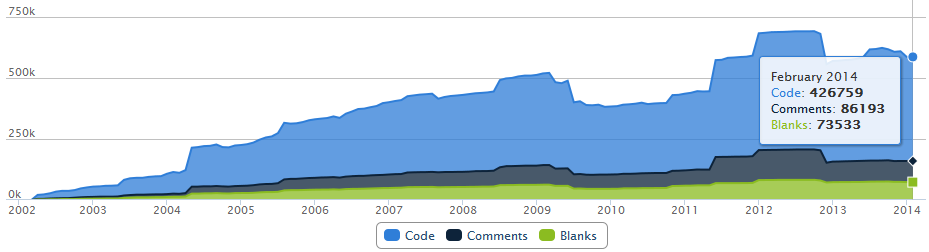
\includegraphics[width=\textwidth]{104_2014_w_Swierczewski_ohloh1.png}
  Figure 1. BOINC project – lines of code (data from 5 February 2014). Source: www.ohloh.net.
\end{figure}

\begin{figure}[b!]
  \centering
  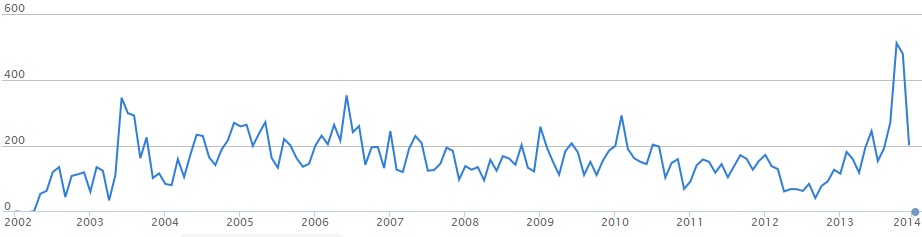
\includegraphics[width=\textwidth]{104_2014_w_Swierczewski_ohloh2.png}
  Figure 2. BOINC project – commits per month (data from 5 February 2014). Source: www.ohloh.net.
\end{figure}

Many projects using BOINC also provides their source code of applications or modules. Many users often try to optimize the application code so that it becomes more afficient . Sometimes such an improved software goes to the administrators of the project, and will be officially added and used as standard on all computers in the system. Also an interesting idea is to announca a competition for the best algorithm and its implementation in a particular programming language. This type of far more `social' solution was used recently in the project OPro\-ject@\-Ho\-me (www.oproject.info) in the subproject Weird Engine, which aims to find the so-called `weird numbers". After two months and receiving several interesting proposals, it turned out that the best solution has been sent by the Frenchman "--- Cedric Den Drijver. Basing on the new concept, a new version of the application has been created, which was several hundred times faster than the previous one. This change significantly contributed to the development of the project OPro\-ject@\-Ho\-me. With it you can now get far more results.

The only conclusion is that sometimes it is worth to describe a problem and ask for international help in finding a solution. If the issue is interesting, then, despite the fact, that the level of knowledge required to solve it, is very large and beyond knowledge of a statistical student, one can expect a response from some part of the world. For the creators of the BOINC projects, development can move in two directions. The first is calculations performed on thousands of computers and other, working on more and more perfect algorithms, which often are written not only by the official developers. Contribution to the project can be achieved by whole society, which forms around the project.

\end{document}
